\documentclass[a4paper,12pt]{report}

\usepackage[brazil]{babel}
\usepackage[utf8]{inputenc}
\usepackage[T1]{fontenc}
\usepackage{listings}
\usepackage{color}
\usepackage{graphicx}

\usepackage[top=2cm,bottom=2.5cm,left=2.5cm,right=2cm]{geometry}
\lstset{basicstyle=\small,breaklines=true,frame=single,numbers=left}

\begin{document}

    \begin{titlepage}
        \begin{center}

            % \large
            UNIVERSIDADE DE SÃO PAULO\\
            Escola Politécnica\\
            Departamento de Computação e Sistemas Digitais
            \vspace{8cm}
            
            \Huge
            \textbf{Compilador Allegri}
            
            \vspace{0.5cm}
            \large
            Projeto Final da Disciplina de Compiladores - PCS 2508
            
            \vspace{2.5cm}
            \Large
            Gabriel Casarin da Silva
            
        \end{center}
        
        \vspace{3.0cm}
        \setlength{\parindent}{10.5cm}
        \large Professor Responsável:

        \setlength{\parindent}{10.5cm}
        Prof. Dr. João José Neto
        

        \begin{center}
            \vfill
            \large
            São Paulo, 2016
        \end{center}
            
    \end{titlepage}
        

    \tableofcontents
    % \renewcommand{\labelitemi}{\textendash}
    \newpage
    \chapter*{Introito}
    \addcontentsline{toc}{part}{Introito}
    O projeto da disciplina PCS 2508 - Linguagens e Compiladores de 2016 consistiu em desenvolver uma linguagem de programação e projetar um compilador para ela. A linguagem desenvolvida foi denominada Barber. O seu compilador, Allegri.

    Por isso, este documento é divido em duas partes. A primeira descreve a linguagem Barber, sua motivação e aspéctos teóricos. A segunda documenta as etapas do desenvolvimento do compilador Allegri.

    Ao final, trazemos uma série de programas-exemplo e de testes dos códigos de máquina gerados pela compilação \textemdash ~ testes estes realizados no simulador de Máquina de von Neumann (MVN).
    
    \addcontentsline{toc}{part}{Um Prelúdio à Linguagem Barber}
    \part*{Um Prelúdio à Linguagem Barber}

    \addcontentsline{toc}{section}{Motivação}
    \section*{Motivação}
    O desafio de se criar uma nova linguagem de programação está no compromisso que deve ser feito entre os recursos que essa linguagem deve suportar, a complexidade de sua sintaxe, o propósito de utilização, o suporte a um ou vários tipos de hardware, eficiência no desenvolvimento de software, legibilidade do código, etc.

    Além disso, deve-se escolher o paradigma (ou paradigmas) que essa linguagem deverá seguir. Um dos paradigmas que obteve grande sucesso desde o seu surgimento é o Paradigma Estrurado. Ele surgiu como reação à necessidade de se desenvolver código com correição, re-utilizável e portável. O projeto de um compilador de uma linguagem estruturada pode ser feito de maneira simplificada, uma vez que há entre a maioria dos comandos daquela e o código de máquina que os implementa traduções diretas.  
    
    Porém, com o progresso do hardware e o avanço das técnicas de engenharia de software, surgiram novos tipos de linguagem para explorar esses novos recursos. Essas linguagens de programação desenvolvidas atualmente são, em sua grande maioria, interpretadas \textemdash ~ ou seja, os programas escritos nessas linguagens são feitos para serem executados em um ambiente de simulação de hardware virtual.

    Das linguagens não interpretadas de propósito geral, apenas duas continuam a ser usadas extensivamente \textemdash ~ C e C++. C vem da época dos processadores unicore, de computação não distribuída. Por isso, não incorpora em si a evolução da computação das últimas décadas, tais como processamento paralelo e distribuído. Mesmo assim, ela ainda é utilizada para desenvolvimento de software embarcado e de sistemas operacionais. C++ continua sendo desenvolvida, porém sua sintaxe complexa implica em compilação ineficiente e demorada. Além disso, sua curva de aprendizado é íngreme e impõe obstáculos ao desenvolvimento de grandes projetos de software.

    Nesse contexto surgiu a linguagem Go. Seu objetivo é ter uma sintaxe simplificada  ao mesmo tempo trazer suporte às novas tendências da Computação. Por isso, o processo de desenvolvimento em Go é ágil e sua compilação, eficiente.

    A linguagem Barber buscou inspirar-se na filosofia que deu origem à linguagem Go. Ela pretende ser uma linguagem didática, ter uma sintaxe compacta, regular e de fácil aprendizado, permitir o desenvolvimento ágil e ter um código legível. Foi projetada para ser compilada para uma Máquina de von Neumann genérica (MVN). 

    \newpage
    \section*{Sintaxe}
    \addcontentsline{toc}{section}{Sintaxe}
    A sintaxe é especificada usando a notação de Wirth:
    \begin{lstlisting}[numbers=none,frame=none]
    DefineFunc       =  "def" Identificador [Tipo] "enter"
                        { DeclaraParam } Bloco .

    DeclaraParametro =  "par" Identificador {, Identificador}
                              Tipo {"[" "]"}.

    DeclaraVariavel  =  "var" Identificador {"," Identificador}
                              Tipo { "[" Numero "]" } .

    Bloco            =  "{" {"enter" [Comando]} "}".

    Comando          =  (DeclaraVariavel
                        | Atribuicao
                        | Return
                        | IF
                        | WHILE
                        ) "enter" {"enter"} .

    IF               =  "if" Teste Bloco
                            { "elif" Teste Bloco }
                            [ "else" Bloco ] .

    WHILE            =  "while" Teste Bloco .

    ConstBool        =  "True" | "False" .

    ExpressaoBool    =  TermoBool { "or" TermoBool } .

    TermoBool        =  FatorBool { "and" FatorBool }.

    FatorBool        =  ConstBool
                        | "not" FatorBool
                        | Operando
                        | "(" ExpressaoBool ")" .

    Expressao        =  ["-"] Termo { ("+" | "-") Termo } .

    Termo            =  Fator { ("*" | "/") Fator } .

    Fator            =  Numero
                        | Operando
                        | "(" Expressao ")" .

    Operando         =  Identificador [
                          "[" Expressao { "," Expressao } "]"
                          | "(" Expressao { "," Expressao } ")"
                        ] .

    Atribuicao       =  Operando "=" (Expressao | ExpressaoBool) .

    Return           =  "return" (Expressao | ExpressaoBool) .

    Comparacao       =  Expressao (
                            ">" | ">=" | "<"| "<=" | "=="| "!="
                        ) Expressao .

    Teste            =  Comparacao | ExpressaoBool .

    Tipo             =  "int"
                        | "char"
                        | "bool" .

    Identificador    =  ("Letra" | "_" )
                        {"Letra" | "Algarismo" | "_"} .

    Numero          =  "Algarismo" {"Algarismo"} .
    \end{lstlisting}

    \subsubsection*{Declaração de Função}
    \addcontentsline{toc}{subsection}{Declaração de Função}
    Uma declaração de função associa um identificador a uma função. Aquela deve ser iniciada com um \textbf{def} seguido de um nome. Caso ela retorne algum valor, deve indicar o tipo de valor que retorna. Caso for um procedimento, não é necessário declarar retorno de tipo \textit{void}. Nas próximas linhas, deve-se declarar os eventuais parâmetros formais que a função dependerá.

    Exemplo de declaração de função:

    \begin{lstlisting}[caption={Declaração de função}]
    def min int
        par x, y int {
        if x < y {
            return x
        }
        return y
    }
    \end{lstlisting}

    \subsubsection*{Declaração de Parâmetros Formais}
    \addcontentsline{toc}{subsection}{Declaração de Parâmetros Formais}
    Uma declaração de parâmetro simples segue a seguinte sintaxe:

    \begin{verbatim}
    DeclaraParametro =  "par" Identificador {, Identificador} Tipo {"[" "]"}. \end{verbatim}
    Tipo pode ser \textbf{int, char} ou \textbf{bool}. Caso o parâmetro seja uma referência a um vetor ou matriz, deve-se seguir o tipo com pares de abre-fecha colchete tantos quantos for o \textit{rank} do objeto (1 para vetor, 2 para matriz).

    Parâmetros formais são declarados logo abaixo da assinatura da função.
    
    \textit{Exemplo 1} ~
     No Listing 1, na linha 2, foram declarados dois parâmetros simples, x e y, de tipo \textbf{int}.

    \textit{Exemplo 2} ~
     Declaração de parâmetro vetor: ~~~\verb|par v int[]|
    
    \textit{Exemplo 3} ~
     Declaração de parâmetro matriz: ~\verb|par m int[][]|

    \subsubsection*{Declaração de Variáveis}
    \addcontentsline{toc}{subsection}{Declaração de Variáveis}
    Uma declaração de variável simples segue a seguinte sintaxe:
    \begin{verbatim}
DeclaraVariavel = "var" Identificador {"," Identificador} Tipo {"[" Numero "]"}. \end{verbatim}
    As declarações de variáveis são muito similares às de parâmetros formais, com exceção de que: (\textit{i}) elas devem ocorrer logo no início do bloco da função, entre o fim da declaração de parâmetros e o início do código; (\textit{ii}) as dimensões de vetores e matrizes precisam ser declarados como números constantes (não há suporte a alocação dinâmica).
    
    \textit{Exemplo 1} ~
     Declarações de variáveis simples são idênticas às de parâmetros formais, apenas com a palavra \textbf{par} trocada por \textbf{var}.

    \textit{Exemplo 2} ~
     Declaração de vetor: ~~~\verb|var v int[10]|
    
    \textit{Exemplo 3} ~
     Declaração de matriz: ~\verb|var m int[5][20]|


    \subsubsection*{Comandos condicionais}
    \addcontentsline{toc}{subsection}{Comandos condicionais}


    \subsubsection*{Comando while}
    \addcontentsline{toc}{subsection}{Comando while}

    % \newpage
    \section*{Como Compilar}
    \addcontentsline{toc}{section}{Como Compilar}
    A estrutura de diretórios do repositório do compilador é como segue:
    \begin{verbatim}
    ./Allegri
    |--- Barber Lang
    |--- comum
    |    +--- automatos
    |--- Meta Compilador
    |--- mvn_build_system
    |    |--- biblioteca
    |    |--- bin
    |    +--- src
    |--- src
    +--- util
    \end{verbatim}

    Diferentemente de outros compiladores, o arquivo com o código-fonte deve ser colocado em um diretório específico \textemdash \space ./Allegri/src \textemdash \space para ser compilado. Para compilar um arquivo \verb|foo.barber|, digite no terminal o seguinte comando:

    \begin{verbatim}
    $ make fonte=foo \end{verbatim}

    Caso o comando acima resulte em sucesso na compilação, o código assembly gerado é posto na pasta mvn\_build\_system/src sob o nome de \verb|foo.asm|. Nesse momento, o programa estará pronto para ser montado e, em seguida, executado na MVN.

    \section*{Ambiente de Execução MVN}
    \addcontentsline{toc}{section}{Ambiente de Execução MVN}
    Após o processo de compilação, faz-se necessária ainda a montagem do código assembly. O montador, linkador e a própria MVN foram obtidos de disciplinas anteriores.
    A máquina em que vamos simular os programas compilados é bem limitada no seu conjunto de instruções. Por isso, tomamos a liberdade de escrever uma pequena biblioteca de sub-rotinas auxiliares, as quais implementam para a MVN as funcionalidades de:
    
    \begin{enumerate}
        \item Operações com tipos booleanos (and, or e not), comparações entre valores, etc.;
        \item Definir o valor das constantes True e False, além de reservar espaço para registradores especiais como FP (\textit{frame pointer}), SP (\textit{stack pointer}) e ACC\_AUX (acumulador auxiliar);
        \item Instruções para leitura e escrita em endereços e relativos tanto a:
            \begin{enumerate}
                \item o \textit{frame pointer} \textemdash~ utilizado para variáveis e parâmetros;
                \item endereços absolutos da área de dados (pointeiros) \textemdash~ utilizado para indexação de vetores e matrizes;
            \end{enumerate}
        \item Alocação de espaço estático na área de dados;
        \item Comandos de Push e Pop na pilha de execução do programa;
    \end{enumerate}

    Eis a estrutura do Ambiente de Execução MVN:
    \begin{verbatim}
    ./mvn_build_system
    |-- biblioteca
    |   |-- boolean.asm
    |   |-- boolean_op.asm
    |   |-- comparacao.asm
    |   |-- const.asm
    |   |-- environment.asm
    |   |-- heap.asm
    |   +-- push_pop.asm
    |-- bin
    |   |-- MLR.jar
    |   |-- mvn.jar
    |   +-- saida.mvn
    |-- Makefile
    |-- saida.mvn -> bin/saida.mvn
    +-- src
    \end{verbatim}

    Quando o comando \verb|make| é executado para compilar um código-fonte, ele automaticamente chama o montador da MVN, depois o seu linkador (para ligar o código compilado com a biblioteca do ambiente de execução) e passa a executar o código pronto. O código de máquina resultante da linkagem é salvo no arquivo ./bin/saida.mvn. Caso se queira apenas executar o montador para o arquivo \verb|bar.asm|, deve-se executar no terminal o seguinte comando:

    \begin{verbatim}
    $ make bar \end{verbatim}

    E para iniciar o simulador MVN,

    \begin{verbatim}
    $ make run \end{verbatim}



    \part*{Compilador Allegri\\\textit{Da capo}}
    \addcontentsline{toc}{part}{Compilador Allegri - Da capo}
    \chapter*{Arquitetura}
    \addcontentsline{toc}{section}{Arquitetura}
    \chapter*{Análise Léxica}
    \addcontentsline{toc}{section}{Análise Léxica}
    \chapter*{Análise Sintática}
    \addcontentsline{toc}{section}{Análise Sintática}
    \chapter*{Análise Semântica e Geração de Código}
    \addcontentsline{toc}{section}{Análise Semântica e Geração de Código}
    \subsection*{Organização da Memória}
    \addcontentsline{toc}{subsection}{Organização da Memória}
    \begin{figure}[h]
        \centering
        \includegraphics[scale=0.75]{OrganizacaoMemoria}
    \end{figure}

    \part*{Testes e Simulações\\\textit{Scherzo}}
    \addcontentsline{toc}{part}{Testes e Simulações - Scherzo}
    Passamos agora a demonstrar o uso da linguagem Barber em diversos exemplos.
    
    \subsection*{Chamada de Sub-rotina}
    \addcontentsline{toc}{section}{Chamada de Sub-rotina}
    Temos duas funções:
    \begin{itemize}
        \item f(int, int) -> int : retorna (p1+7)*(p2+2)
        \item main() -> None : sub-rotina que chama f(10, 20)
    \end{itemize}
    O objetivo deste exemplo é o de demonstrar como funciona o mecanismo de passagem de parâmetros e retorno de valor via pilha de execução.

    Código:
    \begin{lstlisting}
    def f int 
        par p1, p2 int {
        var v3, v4 int

        v4 = 2
        v3 = 7

        return (p1 + v3) * (p2 + v4)
        }

    def main {
        f(10, 20)
        }
    \end{lstlisting}
    Resultado da execução na MVN:
    \begin{figure}[h]
        \centering
        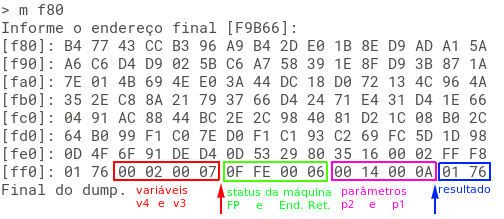
\includegraphics[scale=0.65]{chamada_subrotina}
    \end{figure}

    O dump acima revela como o código fez o gerenciamento da pilha de execução dinâmica durante a "vida" do programa.

    A seta em azul indica a posição da memória em que se encontrava FP (ponteiro de início de frame ou activation record) antes da chamada a f (ou seja, FP da sub-rotina main).
    Conforme os valores reais dos parâmetros formais vão sendo calculados, aqueles vão sendo empilhados de forma a construir uma lista de passagem de parâmetros para a função f por pilha. A sub-rotina terá acesso a esses valores por meio de cálculo de endereços relativos ao seu FP. Cada parâmetro ocupa uma posição de memória com offset bem determinado em relação a FP.

    O conteúdo do retângulo verde representa o estado anterior da sub-rotina main salvo no frame, de modo que seja possível restaurar esse estado após o retorno de f e que a execução de main possa prosseguir como se nada a houvesse interrompido. Primeiramente é salvo o endereço de retorno que está armazenado na primeira posição de memória da sub-rotina main; em segudo lugar, vem o valor de FP antigo (antes de ser atualizado por f).

    A seta em vermelho indica o novo valor de FP, o qual indicará a f onde inicia-se o seu contexto. Ou seja, indica a posição de memória que separa os frames de f e main. Tudo o que estiver além desse novo FP estará sob responsabilidade de f (tais como a alocação de novas variáveis etc.) e o que estiver aquém, está sob responsabilidade de main. A função f acessa os valores dos parâmetros passados por main por meio de acesso a endereços relativos ao seu FP. Bem como armazena suas variáveis locais a partir desse endereço. O valor de retorno de f é posto o mais próximo possível do frame de main. Desse modo procedimento de retorno da sub-rotina é feito de forma mais eficiente e, além disso, o resultado "aparecerá" para main no topo de sua pilha, agilizando o acesso a esse valor.

    Por fim, percebe-se o espaço alocado por f para as suas duas variáveis locais, v3 e v4, as quais armazenam valores constantes e, por isso, como pode-se notar, não têm seus valores alterados durante a execução do programa. Todos os cálculos  são realizados na pilha, porém, sem afetar nenhum conteúdo que lá esteja salvo.
    E last but not least, não se poderia deixar de notar que a sub-rotina f faz o cálculo como o esperado (176hex = 374dec = (10+7)*(20+2)) e armazena-o onde era suposto (como a função main não possui parâmetros nem variáveis, neste caso é a primeira posição de memória da pilha). 

    \subsection*{Expressões Aritméticas com Chamadas Aninhadas a Sub-rotinas: Reentrância}
    \addcontentsline{toc}{section}{Expressões Aritméticas com Chamadas Aninhadas a Sub-rotinas: Reentrância}
    A fim de demonstar o poder que a passagem de parâmetros via pilha de execução dinâmica acrescenta à linguagem, tendo em vista que certas expressões aritméticas podem ser escritas mais concisamente expressando-se os parâmetros de uma sub-rotina em função do resultado de outra, foi escrito o seguinte programa:

    \begin{lstlisting}
    def f int
        par p1, p2 int {
        return (p1 + p2)*2
    }

    def main {
        var a, b int
        b = 4660
        a = 3 + 6*f(3 + f(1, (7 - (1 + 4))), 5)
    }
    \end{lstlisting}

    Esse pequeno programa tem como intuito mostrar o gérmen do conceito de sub-rotina reentrante. Diz-se que uma sub-rotina é reentrante se e somente se a sua área de código for estanque em relação à área de dados. Como consequência, uma mesma porção de programa pode operar sobre áreas da memória de dados distintas - tendo-se que fazer apenas  uma mudança de contexto, claro.

    As vantagens desse esquema são várias. Dentre elas:

    \begin{enumerate}
        \item Uso eficiente da memória de programa (código compartilhado);
        \item Possibilita a implementação de sub-rotinas recursivas;
        \item Maior organização e segmentação da memória do computador;
        \item Dados de uma tarefa não correm o risco de serem alterados quando da execução da mesma sub-rotina por outra tarefa concorrente.
    \end{enumerate}

    O resultado do código compilado é mostrado a seguir:

    \begin{figure}[h]
        \centering
        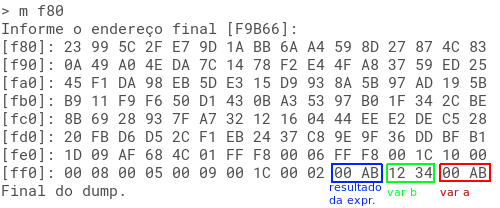
\includegraphics[scale=0.65]{chamada_subrotinas_aninhadas}
    \end{figure}

    Pode-se ver claramente que o resultado da expressão aritmética foi sendo calculado aos poucos, por meio do armazenamento de resultados parciais na pilha. Alguns deles foram sobrescritos conforme a execução do programa avançou. Porém, a ordem em que esses resultados foram calculados segue a mesma dos parâmetros de f. Por isso, f(1, (7 - (1+4))) foi calculado antes, uma vez que o seu resultado era imprescindível ao cálculo total da expresão de atribuição. Ao final, o resultado que foi colocado no topo da pilha (logo após a área das variáveis) foi corretamente atribuído a variável a (a variável b foi criada apenas para mostrar isso mais claramente).
    
    \subsection*{Fatorial: Recursividade}
    \addcontentsline{toc}{section}{Fatorial: Recursividade}
    Um dos exemplos clássicos de computação com recursão é o do cálculo do fatorial de um número. Apresento a seguir a versão desse algoritmo escrito em nossa linguagem:

    \begin{lstlisting}
    def fat int
        par n int {
        if n == 0 {
            return 1
        }
        return n * fat(n-1)
    }

    def main {
        var a, b int
        b = 6
        a = fat(b)
    }
    \end{lstlisting}

    O resultado é mostrado a seguir:
    \newpage
    \begin{figure}[h]
        \centering
        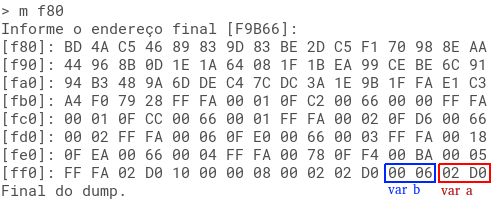
\includegraphics[scale=0.65]{fat_recursao}
    \end{figure}

    Como pode-se perceber, tal tipo de construção consome muita memória. Consumo esse causado pela grande quantidade de dados que precisam ser salvos a cada chamada da função fat.

    Nesse exemplo, calculou-se o fatorial de 6, que resulta 720dec = 2D0hex.

    Note a correta execução da condição de parada (3ª linha), quando n anula-se e tem como resultado o retorno do valor 1.
    
    \subsection*{Fatorial não recursivo}
    \addcontentsline{toc}{section}{Fatorial não recursivo}
    Esse exemplo serve apenas para demonstrar como o programa pode ficar mais enxuto e, portanto, eficiente, caso abandone-se a abordagem de chamada de funções recursivas e venha a se adotar um laço while em vez daquela. De sobra, esse exemplo demonstra o uso do tal comando while:

    \begin{lstlisting}
    def main {
        var a, b int
        a = 1
        b = 6
        while b > 0 {
            a = a * b
            b = b - 1
        }
    }
    \end{lstlisting}

    Segue o resultado:

    \begin{figure}[h]
        \centering
        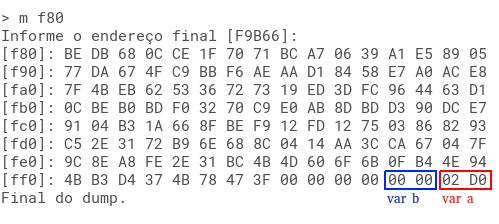
\includegraphics[scale=0.65]{fat_while}
    \end{figure}

    O resultado foi o mesmo do anterior (ufa!). Nota-se que o uso da pilha foi consideravelmente menor, o que mostra que esse programa é mais eficiente. Note o valor final da variável b. Ele coincide com o da condição de parada do loop, como era de se esperar.
    
    \subsection*{Atribuição a Elemento de Vetor}
    \addcontentsline{toc}{section}{Atribuição a Elemento de Vetor}
    
    \subsection*{Somatório de Elementos de Vetor}
    \addcontentsline{toc}{section}{Somatório de Elements de Vetor}

    \begin{lstlisting}
    def somar int
        par v int[] {
        var i int
        var soma int

        soma = 0
        
        i = 0
        while i < len(v) {
            soma = soma + v[i]
            i = i + 1
        }
        
        return soma
    }

    def main {
        var z int[10]
        var soma, i int
        var x int
        
        i = 0
        while i < len(z) {
            z[i] = 2*i + 1
            i = i + 1
        }
        
        soma = somar(z)
        x = soma*2 + 1
    }
    \end{lstlisting}

    \begin{figure}[h]
        \centering
        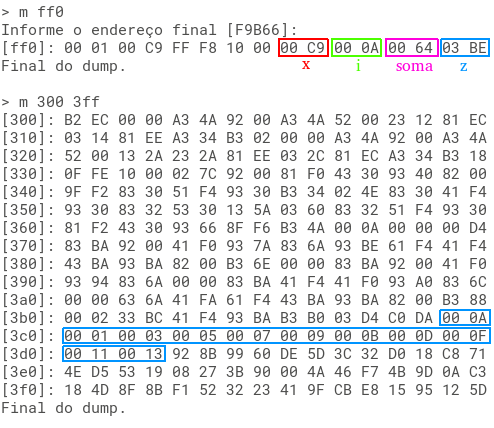
\includegraphics[scale=0.7]{soma_vetor}
    \end{figure}

    \subsection*{Multiplicação de Matrizes}
    \addcontentsline{toc}{section}{Multiplicação de Matrizes}

    \begin{lstlisting}
    def mult
        par m1, m2, mr int[][] {
        var i, j, k, temp int

        i = 0
        while i < 2 {
            j = 0
            while j < 1 {
                k = 0
                temp = 0
                while k < 2 {
                    temp = temp + m1[i, k]*m2[k, j]
                    k = k + 1
                }
                mr[i, j] = temp
                j = j + 1
            }
            i = i + 1
        }

    }

    def main {
        var x int[2][2]
        var y, z int[2][1]

        x[0, 0] = 11
        x[0, 1] = 1
        x[1, 0] = 12
        x[1, 1] = 8

        y[0, 0] = 14
        y[1, 0] = 5

        mult(x, y, z)

    }
    \end{lstlisting}

    \begin{figure}[h]
        \centering
        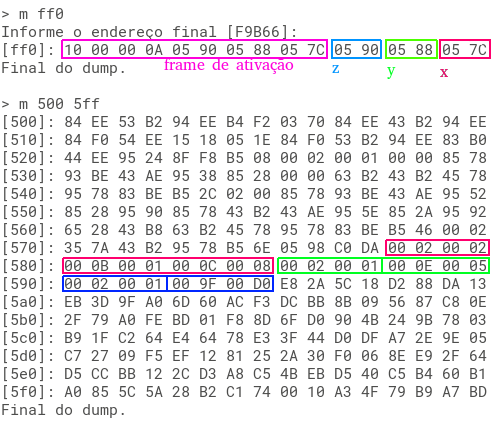
\includegraphics[scale=0.65]{mult}
    \end{figure}

    \chapter*{Finale}
    \addcontentsline{toc}{part}{Finale}
\end{document}
